% Capítulo 3: ordem de avaliação de uma expressão com operadores de vários tipos.
\documentclass[border=4pt]{standalone}
\usepackage[utf8]{inputenc}
\usepackage[T1]{fontenc}
% Estilo comum dos fluxogramas e diagramas de blocos.
\usepackage{tikz}
\usetikzlibrary{arrows.meta, positioning, calc, shapes.geometric, shapes.misc}
\definecolor{navy}{RGB}{23,45,80}
\definecolor{laranja}{RGB}{250,110,29}
\definecolor{cinzalogo}{RGB}{107,114,126}
\definecolor{azul}{RGB}{205,222,247}
\tikzset{
  base/.style={draw=navy, line width=0.9pt, font=\sffamily\small, align=center, inner sep=4pt},
  terminal/.style={base, rounded rectangle, fill=laranja!45, draw=laranja, minimum width=20mm, minimum height=7mm},
  processo/.style={base, rectangle, fill=laranja!12, minimum width=28mm, minimum height=8mm},
  decisao/.style={base, diamond, aspect=2.2, fill=azul, inner sep=1pt, minimum width=30mm},
  es/.style={base, trapezium, trapezium left angle=72, trapezium right angle=108,
             fill=white, minimum width=26mm, minimum height=8mm, trapezium stretches body},
  fluxo/.style={-{Stealth[length=2.2mm]}, navy, line width=0.9pt},
  rotulo/.style={font=\sffamily\small\bfseries, text=navy},
  legenda/.style={font=\sffamily\scriptsize, text=cinzalogo},
  resposta/.style={font=\sffamily\scriptsize\bfseries, text=navy},
}

\tikzset{
  expr/.style={font=\ttfamily\small, text=navy, anchor=west},
  passo/.style={font=\sffamily\scriptsize, text=laranja, anchor=west},
  destaque/.style={fill=laranja!30, rounded corners=2pt, inner sep=1.5pt},
}
\begin{document}
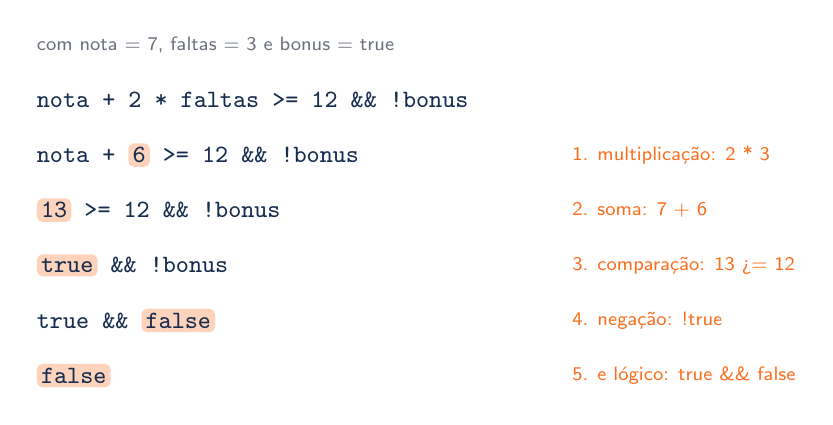
\begin{tikzpicture}
  \node[legenda, anchor=west] at (0, 0.7) {com nota = 7, faltas = 3 e bonus = true};
  \node[expr] at (0, 0) {nota + 2 * faltas >= 12 \&\& !bonus};
  \node[expr] at (0, -0.7) {nota + \tikz[baseline]\node[destaque, anchor=base]{6}; >= 12 \&\& !bonus};
  \node[passo] at (6.8, -0.7) {1. multiplicação: 2 * 3};
  \node[expr] at (0, -1.4) {\tikz[baseline]\node[destaque, anchor=base]{13}; >= 12 \&\& !bonus};
  \node[passo] at (6.8, -1.4) {2. soma: 7 + 6};
  \node[expr] at (0, -2.1) {\tikz[baseline]\node[destaque, anchor=base]{true}; \&\& !bonus};
  \node[passo] at (6.8, -2.1) {3. comparação: 13 >= 12};
  \node[expr] at (0, -2.8) {true \&\& \tikz[baseline]\node[destaque, anchor=base]{false};};
  \node[passo] at (6.8, -2.8) {4. negação: !true};
  \node[expr] at (0, -3.5) {\tikz[baseline]\node[destaque, anchor=base]{false};};
  \node[passo] at (6.8, -3.5) {5. e lógico: true \&\& false};
\end{tikzpicture}
\end{document}
